\bab{HASIL DAN PEMBAHASAN}
\subbab{Pengumpulan Dokumen Email}
Korpus yang digunakan pada penelitian ini adalah public email corpus yang disediakan oleh Spamassasin dengan kode prefix “20030228”. Korpus ini terdiri atas 6.047 pesan email yang sudah diklasifikasikan sebelumnya dengan komposisi:
\begin{itemize}
	\item 3900 easy-ham, yaitu pesan ham yang dapat dibedakan dengan mudah dari pesan spam karena tidak banyak mengandung ciri-ciri yang dimiliki oleh pesan spam.
	\item 250 hard-ham, yaitu pesan bertipe ham namun mengandung cukup banyak feature yang biasa terdapat pada pesan spam sehingga agak sulit diklasifikasikan.
	\item 1897 spam, yaitu pesan yang masuk dalam kategori spam.
\end{itemize}

Dari masing-masing kategori, secara acak diambil sebanyak 70\% sebagai data latih dan sisanya digunakan data uji. Pesan yang memiliki label easy-ham dan hard-ham digabungkan ke dalam satu kategori yaitu ham. Dengan demikian, dokumen email tersebut diklasifikasikan ke dalam dua kategori yaitu spam dan ham dengan komposisi:
\begin{itemize}
	\item Total dokumen ham 4150, sebanyak 2905 dokumen digunakan sebagai data latih dan 1245 dokumen digunakan sebagai data uji.
	\item Total dokumen spam 1897, sebanyak 1328 dokumen digunakan sebagai data latih dan 569 dokumen digunakan sebagai data uji.
\end{itemize}

Hasil pengamatan menunjukkan dokumen spam rata-rata mempunyai ukuran data yang lebih besar dibandingkan dengan dokumen ham. Ukuran terbesar dari dokumen ham adalah 301 KB, sedangkan untuk dokumen spam adalah 232 KB. Besar ukuran dokumen email tergatung dari isi yang terdapat di dalam dokumen. Dokumen email dengan content-type multipart biasanya menghasilkan ukuran data yang lebih besar dibandingkan dengan singlepart.

\subbab{Ekstraksi Dokumen Email}
Langkah ekstraksi dokumen dilakukan untuk memecah dokumen email menjadi bagian-bagian yang lebih kecil. Langkah ini diperlukan karena tidak semua bagian email digunakan untuk tahapan selanjutnya. Struktur header seperti sender, return path, dan X-mailer hanya muncul pada beberapa dokumen email sehingga tidak bagus digunakan sebagai penciri. Subject email merupakan salah satu bagian email yang baik digunakan sebagai penciri (\cite{SAHAMI}). Bagian struktur email yang digunakan untuk langkah selanjutnya adalah subject dan body (plain text dan HTML text).

Ekstraksi dokumen menggunakan library mailparse\footnote{Dapat diunduh pada http://pecl.php.net/package/mailparse} yang telah tersedia untuk bahasa pemrograman php. Hasil pengamatan menunjukkan content plain text paling banyak ditemukan pada dokumen easy-ham, sedangkan HTML text banyak ditemukan pada dokumen hard-ham dan spam.

\subbab{Praproses}
Tahap tokenisasi dilakukan pada bagian email yang digunakan. Dalam tahap tokenisasi data latih diperoleh 67612 token. Seluruh token tersebut disaring dengan membuang kata-kata yang terdapat dalam daftar stopword sehingga diperoleh token sebanyak 67172. Dapat disimpulkan bahwa hanya sebanyak 0.7\% dari seluruh token data latih merupakan stopword. Dengan menggunakan seleksi fitur chi-square dan taraf $\alpha$ = 0.01, token akhir yang dijadikan sebagai vocabulary adalah 3866 token atau 5.8\% dari total token setelah pembuangan stopword. Tabel \ref{tab:jumlahToken} menunjukkan jumlah token yang dihasilkan pada setiap langkah praproses. Sebanyak 2273 token terdapat pada kelas ham dan spam seperti kata “absolutely”, “account” dan “address” termasuk tag-tag HTML. Sedangkan sebanyak 690 token hanya terdapat pada kelas ham dan 882 token hanya terdapat pada kelas spam. Gambar \ref{fig:komposisitoken} menunjukkan komposisi jumlah token terhadap kelas dari hasil seleksi fitur.
\begin{table*}[h!]
	\begin{center}
		\caption{Jumlah token yang dihasilkan}
		\label{tab:jumlahToken}
		\begin{tabular}{l r}
			\hline
			Tahapan~~~~~~~~~~&~~~~~~~~~~Jumlah Token \\
			\hline
			Tokenisasi &67612\\
			Membuang Stopword &67172\\
			Seleksi Fitur&3866\\
			\hline
		\end{tabular}
	\end{center}
\end{table*}
\begin{figure*}[h!]
	\centering
	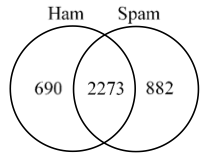
\includegraphics[width=130pt]{hamspam.png}
	\caption{Komposisi jumlah token hasil tahap seleksi fitur}
	\label{fig:komposisitoken}
\end{figure*}

\subbab{Fungsi Klasifikasi Naive Bayes}
Setelah melewati langkah praproses, langkah selanjutnya adalah membuat fungsi klasifikasi yang dapat memetakan dokumen ke dalam kategori tertentu. Pada model Multivariate Bernoulli, pendugaan parameter setiap term dihitung menggunakan persamaan (\ref{eq:peluangNBbernoulli}). Peluang dari pendugaan parameter Multivariate Bernoulli bergantung pada nilai document frequency (DF). Semakin besar nilai DF maka semakin besar pula peluangnya. Tabel 6 menunjukkan lima term urutan tertinggi hasil pendugaan parameter Multivariate Bernoulli berdasar pada nilai DF dan peluangnya. Tabel \ref{tab:limaTermMultivar} menunjukkan pada kelas ham, jika dibandingkan term ‘listinfo’ yang bernilai DF 1839 menghasilkan peluang sebesar 0.633, sedangkan untuk term ‘wrote’ dengan nilai DF 1230 menghasilkan peluang yang lebih kecil yaitu sebesar 0.423.
\begin{table*}[h!]
	\begin{center}
		\caption{Lima term hasil pendugaan pada Multivariate Bernoulli}
		\label{tab:limaTermMultivar}
		\begin{tabular}{l r r | l r r}
			\hline
			\multicolumn{3}{c|}{Kelas Ham}&\multicolumn{3}{c}{Kelas Spam}\\
			\hline
			Term&DF&Peluang&Term&DF&Peluang\\
			\hline
			listinfo&1839&0.633&html&758&0.571\\
			list&1619&0.558&email&729&0.549\\
			mailman&1617&0.557&click&721&0.543\\
			www&1611&0.555&href&690&0.520\\
			wrote&1230&0.423&body&671&0.505\\
			\hline
		\end{tabular}
	\end{center}
\end{table*}

Pada model Multinomial NB, pendugaan parameter dihitung menggunakan persamaan (\ref{eq:peluangNBmultinom}). Berbeda dengan model Multivariate Bernoulli, nilai peluang model Multinomial NB dipengaruhi oleh nilai TF (term frequency). Semakin tinggi nilai TF maka semakin besar pula peluangnya. Tabel \ref{tab:limaTermMultinom} menunjukkan lima term urutan tertinggi hasil pendugaan parameter Multinomial NB berdasar pada nilai TF dan peluangnya. Tabel \ref{tab:limaTermMultinom} menunjukkan pada kelas ham, jika dibandingkan term ‘width yang bernilai TF 16815 menghasilkan peluang sebesar 0.038, sedangkan untuk term ‘src’ dengan nilai TF 9340 menghasilkan peluang yang lebih kecil yaitu sebesar 0.021. Pendugaan $\hat{P}(c)$ untuk setiap model bernilai sama yaitu $\hat{P}(ham)$=0.686 sedangkan $\hat{P}(spam)$=0.314.
\begin{table*}[h!]
	\begin{center}
		\caption{Lima term hasil pendugaan pada Multinomial NB}
		\label{tab:limaTermMultinom}
		\begin{tabular}{l r r | l r r}
			\hline
			\multicolumn{3}{c|}{Kelas Ham}&\multicolumn{3}{c}{Kelas Spam}\\
			\hline
			Term&TF&Peluang&Term&TF&Peluang\\
			\hline
		width&16815&0.038&font&27602&0.090\\
		www&12055&0.027&size&10335&0.033\\
		font&11042&0.025&width&7855&0.025\\
		height&9598&0.022&color&7892&0.025\\
		src&9340&0.021&face&7594&0.024\\
			\hline
		\end{tabular}
	\end{center}
\end{table*}

\subbab{Evaluasi}
Proses pengujian model klasifikasi dilakukan menggunakan
yang terdiri dari 1245 dokumen ham dan 569 dokumen spam. Pengujian menggunakan pendugaan parameter yang telah dibuat pada tahap fungsi klasifikasi. Persamaan (\ref{eq:peluangNBbernoulli}) digunakan pada pengujian model Multivariate Bernoulli sedangkan (\ref{eq:peluangNBmultinom}) digunakan untuk menguji model Multinomial NB. Perhitungan (\ref{eq:peluangNBbernoulli}) dan (\ref{eq:peluangNBmultinom}) menghasilkan nilai 0 karena nilai peluang yang dihasilkan sangat kecil. Oleh karena itu, untuk mengatasi hal tersebut semua nilai pendugaan parameter dijadikan log sehingga persamaan (\ref{eq:peluangNBbernoulli}) menjadi:
\begin{equation*}
\log(P(c|d))\propto \log(\hat{P}(c))+\sum_{t_i\in \mathbb{V}}\log(\hat{P}(U_i=e_i|c))
\end{equation*}
\noindent sedangkan persamaan (\ref{eq:peluangNBmultinom}) menjadi:
\begin{equation*}
\log(P(c|d))\propto \log(\hat{P}(c))+\sum_{1\leq k\leq n_d}\log(\hat{P}(X=t_k|c))
\end{equation*}

Pada semua dokumen uji dilakukan pengujian terhadap setiap model klasifikasi baik sebelum dan sesudah menggunakan seleksi fitur chi-square. Hasil pengujian dalam bentuk confussion matrix terdapat pada lampiran 1. Akurasi tertinggi dicapai model Multinomial NB tanpa seleksi fitur chi-square dengan tingkat akurasi sebesar 95.31\%. Model Multivariate Bernoulli tanpa seleksi fitur chi-square memiliki tingkat akurasi terendah yaitu sebesar 89.69\%. Secara keseluruhan, model Multinomial NB menunjukkan tingkat akurasi yang lebih tinggi, baik menggunakan seleksi fitur atau tidak. Gambar \ref{fig:akurasimodel} menunjukkan tingkat akurasi dari model klasifikasi yang telah dibuat.
\begin{figure*}[h!]
	\centering
	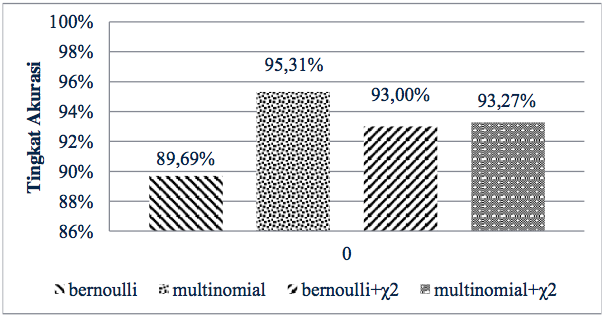
\includegraphics[width=400pt]{akurasimodel.png}
	\caption{Tingkat akurasi setiap model klasifikasi}
	\label{fig:akurasimodel}
\end{figure*}

Gambar \ref{fig:seleksifitur} menunjukkan pengaruh dari seleksi fitur terhadap model klasifikasi. Dengan menggunakan seleksi fitur chi-square, terjadi penuruan akurasi sebesar 1.98\% pada model Multinomial NB. Hal ini berbanding terbalik pada model Multivariate Bernoulli yang mengalami peningkatan akurasi sebesar 3.31\%. Banyaknya vocabulary yang digunakan mempengaruhi turun-naiknya akurasi model klasifikasi. Multivariate Bernoulli lebih baik jika vocabulary yang digunakan berjumlah sedikit, sedangkan untuk vocabulary dalam jumlah banyak, Multinomial NB menghasilkan tingkat akurasi yang lebih baik.
\begin{figure*}[h!]
	\centering
	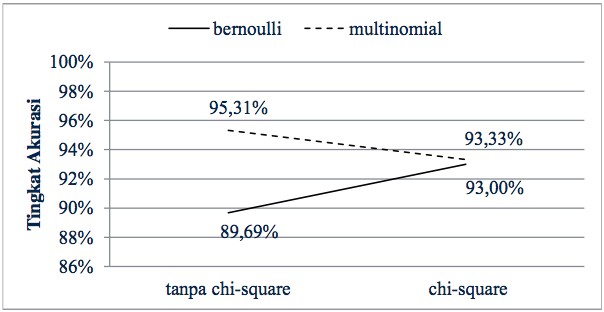
\includegraphics[width=400pt]{seleksifitur.png}
	\caption{Pengaruh seleksi fitur terhadap model klasifikasi}
	\label{fig:seleksifitur}
\end{figure*}
\begin{figure*}[h!]
	\centering
	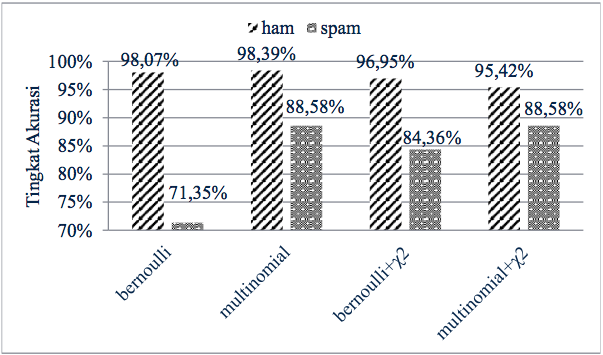
\includegraphics[width=400pt]{akurasihamspam.png}
	\caption{Tingkat akurasi ham dan spam setiap model klasifikasi}
	\label{fig:akurasihamspam}
\end{figure*}

Model Multinomial NB tanpa seleksi fitur chi-square sangat baik dalam mengenali dokumen ham dengan tingkat akurasi 98.39\%. Sedangkan dalam mengenali dokumen spam, model Multinomial NB dengan seleksi fitur chi-square dan tanpa seleksi fitur sama-sama menghasilkan akurasi yang terbaik yaitu sebesar 88.58\%. Gambar \ref{fig:akurasihamspam} menunjukkan tingkat akurasi ham dan spam setiap model klasifikasi. Setiap model klasifikasi menunjukkan tingkat akurasi ham selalu lebih baik dibandingkan dengan akurasi spam.

